\documentclass[9pt]{beamer}
\usepackage{amsmath,amsthm,amssymb,bm}   
\usepackage{algorithm,algorithmic}
\usepackage{hyperref}
\usepackage{color}
\usepackage{subfigure}                
\usepackage{animate}
\usepackage{cite}
\setbeamertemplate{navigation symbols}{}     % 取消底部固有的导航条
\usetheme{metropolis}          
\graphicspath{{figures/}}                    % 图片文件夹
 %====================================自定义命令=======================
\def\mb{\mathbf}
\def\half{\frac{1}{2}}
\def\veps{\varepsilon}
\def\dsp{\displaystyle}
\def\cal{\mathcal}
\def\bm{\boldsymbol}
\newcommand{\dps}{\displaystyle}
\newcommand{\bs}{\boldsymbol}
\newcommand{\pt}{\partial}
\newcommand{\wt}{\widetilde}
\newcommand{\vph}{\varphi}
\newcommand{\D}{\mathrm{d}}
\newcommand{\e}{\varepsilon}
\newtheorem{thm}{Theorem}
\newtheorem{conj}{Conjecture}
\newtheorem{cor}{Corollary}
\newtheorem{defi}{Definition}
\newtheorem{exer}{Exercise}
\newtheorem{lem}{Lemma}
\newtheorem{prop}{Proposition}
\newtheorem{rmk}{Remark}
\newtheorem{sol}{Solution}
\newtheorem{assump}{Assumption}
\DeclareMathOperator*{\argmin}{argmin}
 %====================================自定义命令=======================
\AtBeginSection[]                    
{
        \begin{frame}<beamer>{Contents}
                \tableofcontents[currentsection]
        \end{frame}
}

\setbeamertemplate{bibliography item}[text]

\begin{document}

%%------title -------------------------------------------
    \title{The Scalar Auxiliary Variable Approach for gradient flows}
    \author{Ding Zhao}
    \institute{Wuhan University}
    \date{\today}
    \titlegraphic{
\includegraphics[height=1.0cm]{whulogo.eps}}
    \frame{\titlepage}
\logo{
\includegraphics[height=0.08\textwidth]{whulogo.eps}}

%%-------Content------------------------------------------
\section{Phase Field Recap}

\begin{frame}{Definition}
Given a free energy functional $\mathcal E(\phi(x))$
$$\left\{
\begin{aligned}
\phi_t &= \mathcal{G} \mu \\
\mu &= \frac{\delta \mathcal E}{\delta \phi} \\
\end{aligned}
\right.$$

In the above,  operator $\mathcal G$ gives the dissipation mechanism:
\begin{itemize}
\item{$L^2$ gradient flows when $\mathcal G = -I$} (Allen-Cahn)
\item{$H^{-1}$ gradient flow when $\mathcal G = \Delta$} (Cahn-Hiliard)
 \item{$H^{-\alpha}$ gradient flow when $\mathcal G = -(-\Delta)^{\alpha}$ with $0 < \alpha < 1$}
\end{itemize}
In this talk, we choose periodic boundary conditions or  homogeneous Neumann boundary conditions. % such that boundary terms vanish when integrated by parts.
\end{frame}

\begin{frame}{Dissipation}
As long as $\mathcal G$ is non-positive, the free energy is non-increasing:
$$\frac{\mathrm{d} \mathcal{E}(\phi)}{\mathrm{d} t}=\frac{\delta \mathcal{E}}{\delta \phi} \cdot \frac{\partial \phi}{\partial t}=(\mu, \mathcal{G} \mu) \leq 0$$

In this talk, we consider $\mathcal G$ is non-positive, linear and independent of $\phi$.
\end{frame}

\begin{frame}{Free Energy Functional}
Usually, the free energy functional contains a quadratic term, which we write explicitly as
$$\mathcal{E}(\phi)=\frac{1}{2}(\phi, \mathcal{L} \phi)+\mathcal{E}_{1}(\phi)$$
where $\mathcal L$ is a symmetric non-negative linear operator (independent of $\phi$), and $\mathcal{E}_{1}(\phi)$ are nonlinear but with only lower-order derivatives than $\mathcal L$. We take $\mathcal E_1(\phi) = \int_{\Omega} F(\phi) dx$
\end{frame}

\begin{frame}{Existing Approaches}
\begin{itemize}
\item{Convex Splitting Approach

Assume $F(\phi)= F_c(\phi) - F_e(\phi)$ with $F_{c}^{\prime \prime}(\phi), F_{e}^{\prime \prime}(\phi) \geq 0$.
$$\left\{
\begin{aligned}
\frac{\phi^{n+1}-\phi^{n}}{\delta t}&=\mathcal G \mu^{n+1} \\
\mu^{n+1}&=\mathcal L \phi^{n+1}+\left(F_{c}^{\prime}\left(\phi^{n+1}\right)-F_{e}^{\prime}\left(\phi^{n}\right)\right) 
\end{aligned}
\right.$$
}
\item{Stablized Approach

Introduce stabilization term $S$ to balance nonlinear term.
$$\left\{
\begin{aligned}
\frac{1}{\delta t}\left(\phi^{n+1}-\phi^{n}\right)&=\mathcal G \mu^{n+1} \\
\mu^{n+1}&=\mathcal L \phi^{n+1}+S\left(\phi^{n+1}-\phi^{n}\right)+F^{\prime}\left(\phi^{n}\right)
\end{aligned}
\right.$$
}
\item{Invariant energy quadratization(IEQ)

Introduce  a Lagrange multiplier  $q(t, x ; \phi)=\sqrt{F(\phi)+C_{0}}$.
$$\left\{
\begin{aligned}
\phi_{t} &=\mathcal G \mu \\
\mu &=\mathcal L \phi+\frac{q}{\sqrt{F(\phi)+C_{0}}} F^{\prime}(\phi) \\
q_{t} &=\frac{F^{\prime}(\phi)}{2 \sqrt{F(\phi)+C_{0}}} \phi_{t}
\end{aligned}
\right.$$
}
\end{itemize}
\end{frame}

\section{SAV Approach}

\subsection{Main Idea}

\begin{frame}{SAV}
Assume $\mathcal E_1(\phi)) = \int_{\Omega} F(\phi)dx$ is bounded from below, i.e., $\mathcal E_1(\phi) \geq -C_0$, introduce a scalar auxiliary variable $r(t) = \sqrt{\mathcal E_1(\phi) + C_0}$.
$$\left\{
\begin{aligned} \phi_t &=\mathcal G \mu \\ 
\mu &=\mathcal L \phi+\frac{r(t)}{\sqrt{\mathcal E_{1}[\phi]+C_{0}}} F^{\prime}(\phi) \\ 
r_t &=\frac{1}{2 \sqrt{\mathcal E_{1}[\phi]+C_{0}}} \int_{\Omega} F^{\prime}(\phi) \phi_{t} d x 
\end{aligned}
\right.$$

Taking the inner products of the above with $\mu, \phi_t$ and $2r$ respectively, one can obtain the modified energy dissipation law:
$$
\frac{d}{d t}\left[(\phi, \mathcal{L} \phi)+r^{2}\right]=(\mu, \mathcal{G} \mu)
$$
\end{frame}

\subsection{Numerical Schemes}

\begin{frame}{First-Order Scheme(1)}
$$\left\{
\begin{aligned}
\frac{\phi^{n+1}-\phi^{n}}{\Delta t} &=\mathcal{G} \mu^{n+1} \\
\mu^{n+1} &=\mathcal{L} \phi^{n+1}+\frac{r^{n+1}}{\sqrt{\mathcal{E}_{1}(\phi^{n})+C_0}} F^{\prime}(\phi^n)\\
\frac{r^{n+1}-r^{n}}{\Delta t} &=\frac{1}{2 \sqrt{\mathcal{E}_{1}(\phi^{n})+C_0}} \int_{\Omega} F^{\prime}(\phi^n)\frac{\phi^{n+1}-\phi^{n}}{\Delta t} dx
\end{aligned}
\right.$$

From the above we have
$$
\frac{\phi^{n+1}-\phi^{n}}{\Delta t}=\mathcal{G}\left[\mathcal{L} \phi^{n+1}+\frac{F^{\prime}(\phi)}{\sqrt{\mathcal{E}_{1}(\phi^{n})+C_0}}\left(r^{n}+\int_{\Omega} \frac{F^{\prime}(\phi)}{2 \sqrt{\mathcal{E}_{1}(\phi^{n})+C_0}}\left(\phi^{n+1}-\phi^{n}\right) dx \right)\right]
$$
\end{frame}

\begin{frame}{First-Order Scheme(2)}
denote $b^n = \frac{F^{\prime}(\phi^n)}{\sqrt{\mathcal{E}_{1}(\phi^{n})+C_0}}$,
$$\Rightarrow
(I-\Delta t \mathcal{G L}) \phi^{n+1}-\frac{\Delta t}{2} \mathcal{G}b^{n}\left(b^{n}, \phi^{n+1}\right)=\phi^{n}+r^{n} \mathcal{G} b^{n}-\frac{\Delta t}{2}\left(b^{n}, \phi^{n}\right) \mathcal{G} b^{n} \triangleq c^n$$

Multiply it with $(I-\Delta t \mathcal{G L})^{-1}$ and then take inner product with $b^n$
$$\Rightarrow
\left(b^{n}, \phi^{n+1}\right)+\frac{\Delta t}{2} \gamma^{n}\left(b^{n}, \phi^{n+1}\right)=\left(b^{n},(I-\Delta t \mathcal{G L})^{-1} c^{n}\right)$$
where $\gamma^{n}=-\left(b^{n},(I-\Delta t \mathcal{G} \mathcal{L})^{-1} \mathcal{G} b^{n}\right)=\left(b^{n},\left(-\mathcal{G}^{-1}+\Delta t \mathcal{L}\right)^{-1} b^{n}\right)>0$

hence
$\left(b^{n}, \phi^{n+1}\right)=\frac{\left(b^{n},(I-\Delta t \mathcal{G L})^{-1} c^{n}\right)}{1+\Delta t \gamma^{n} / 2}$
\end{frame}

\begin{frame}{First-Order Scheme(3)}
To summarize, one can implement the first order SAV with following steps:
\begin{enumerate}
\item{compute $b^n$ and $c^n$}
\item{compute $(b^n,\phi^{n+1})$}
\item{compute $\phi^{n+1}$}
\end{enumerate}
Note that in 2 and 3 of the above procedure, one only need to solve, twice, a linear equation with constant coefficients of the form
$$(I-\Delta t \mathcal{G L}) x = b$$
\end{frame}

\begin{frame}{BDF2}
$$\left\{
\begin{aligned}
 \frac{3 \phi^{n+1}-4 \phi^{n}+\phi^{n-1}}{2 \Delta t} &=\mathcal{G} \mu^{n+1}, \\ \mu^{n+1} &=\mathcal{L} \phi^{n+1}+\frac{r^{n+1}}{\sqrt{\mathcal{E}_{1}(\bar{\phi}^{n+1})+C_0}} F^{\prime}(\bar{\phi}^{n+1}) \\ 3 r^{n+1}-4 r^{n}+r^{n-1} &=\int_{\Omega} \frac{F^{\prime}(\bar{\phi}^{n+1})}{2 \sqrt{\mathcal{E}_{1}(\bar{\phi}^{n+1})+C_0}}\left(3 \phi^{n+1}-4 \phi^{n}+\phi^{n-1}\right) dx
 \end{aligned}
\right.$$

Here $\bar{\phi}^{n+1}$ can be any explicit approximation of $\phi^{n+1}$ with an error of $\mathcal O(\Delta t^2)$.

With similar procedure as first order scheme, one can obtain the iteration format. Each iteration requires solving two linear equations with constant coefficients of the form of $$(I-\Delta t \mathcal{G L}) x = b$$

\end{frame}

\begin{frame}{Crank-Nicolson scheme}
The semi-implicit BDF2 can be replaced by semi-implicit Crank–Nicolson scheme.
\end{frame}

\section{Numerical Experiments}

\subsection{Finite Difference Schemes for Cahn-Hiliard Equation}
\begin{frame}{Problem}
Consider free energy functional $\mathcal E(\phi) = \int_{\Omega} \left[ \frac{\varepsilon^2}{2}|\nabla \phi|^2 + \frac{(1-\phi^2)^2}{4} \right]dx$

One can obtain Cahn-Hiliard Equation from it
$$\left\{
\begin{aligned}
\phi_t &= \Delta \mu \\
\mu &= -\varepsilon^2\nabla^2\phi +\phi^3 - \phi\\
\end{aligned}
\right.$$
I chose Neumann boundary conditions $\frac{\partial c}{\partial n}=0=\frac{\partial \omega}{\partial n}$.
\end{frame}

\begin{frame}{Finite Difference Scheme}
For the first equation I used implicit Euler scheme
$$\phi^{n}- \frac{\Delta t}{h^2} D \mu^{n}-\phi^{n-1}=0$$
where the matrix $D$ is the central-difference Laplacian with Neumann boundary conditions.

For the second equation, I considered five different schemes of the form:
$$\mu^{n}+\frac{\epsilon^{2}}{h^{2}} D \phi^{n}-\Phi^{n}=0$$
where $\Phi^n$ is a discretization of the free energy term $F^{\prime}(\phi)$.
\end{frame}

\begin{frame}{Five Finite Difference Schemes}
Depend sensitively on the discretization of the nonlinear term $\Phi^n$, and so I considered the following possibilities:
$$
\begin{array}{l}
\Phi^{n}=\left(\phi^{n-1}\right)^{2} \phi^{n}-\phi^{n-1} \\
\Phi^{n}=\left(\phi^{n-1}\right)^{3}-3 \phi^{n-1}+2 \phi^{n} \\
\Phi^{n}=3\left(\phi^{n-1}\right)^{2} \phi^{n}-2\left(\phi^{n-1}\right)^{2} \phi^{n-1}-\phi^{n}, \\
\Phi^{n}=\left(\phi^{n}\right)^{3}-\phi^{n-1} \\
\Phi^{n}=\left(\phi^{n}\right)^{3}-\phi^{n}
\end{array}
$$
\end{frame}

\begin{frame}{Linear Schemes}
The first three schemes result in  linear system of the form:
$$
\left[\begin{array}{cc}
I & -\mu D \\
R_{n} & I
\end{array}\right]\left[\begin{array}{c}
\phi^{n} \\
\mu^{n}
\end{array}\right]=\left[\begin{array}{c}
\phi^{n-1} \\
b_{n}
\end{array}\right]
$$
where
$$
R_{n}=\left\{\begin{array}{l}
\epsilon^{2} / h^{2} D-\phi_{n-1}^{2}, \\
\epsilon^{2} / h^{2} D-2 I, \\
\epsilon^{2} / h^{2} D-3 \phi_{n-1}^{2}+I
\end{array}\right.
$$
$$
b_{n}=\left\{\begin{array}{l}
-\phi^{n-1} \\
-3 \phi^{n-1}+\left(\phi^{n-1}\right)^{3} \\
-2\left(\phi^{n-1}\right)^{3}
\end{array}\right.
$$
\end{frame}

\begin{frame}{Nonliear Schemes}
The last two schemes take the form of vector systems:
$$
g_{n}=\left[\begin{array}{c}
\phi^{n}- \frac{\Delta t}{h^2} D \mu^{n}-\phi^{n-1} \\
f\left(\phi^{n}, \phi^{n-1}\right)+\mu^{n}
\end{array}\right]=\left[\begin{array}{l}
0 \\
0
\end{array}\right]
$$
$g_n$ has Jacobian $J_n$:
$$
J_{n}=\left[\begin{array}{cc}
I & -\frac{\Delta t}{h^2}  D \\
\partial f / \partial \phi^{n} & I
\end{array}\right]
$$
where the partial derivative term for the two schemes is:
$$
\frac{\partial f}{\partial c^{n}}=\left\{\begin{array}{l}
\epsilon^{2} / h^{2} D-3 \phi_{n}^{2} \\
\epsilon^{2} / h^{2} D-3 \phi_{n}^{2}+I
\end{array}\right.
$$
When implementing Newton’s method, at each time-step n I used the previous iterates $\phi^{n-1}$ and $\mu^{n-1}$ as starting guesses for the roots, and computed the Newton step s by solving the linear system
$$J_ns=-g_n$$
\end{frame}

\begin{frame}{Numerical Results}
I ran the above five schemes on $[0,1]^2 \times 200\Delta t $, with smooth initial conditions $\phi_0(x,y) = cos(2\pi x)cos(\pi y)$, and the mesh resolution was set $64\times64$.
%\animategraphics[autoplay,
%					loop,
%					controls,
%					width=.5\textwidth]{15}{./figures/cahn-hiliard/ex1/}{001}{200}

\begin{figure}[H]
  \centering
  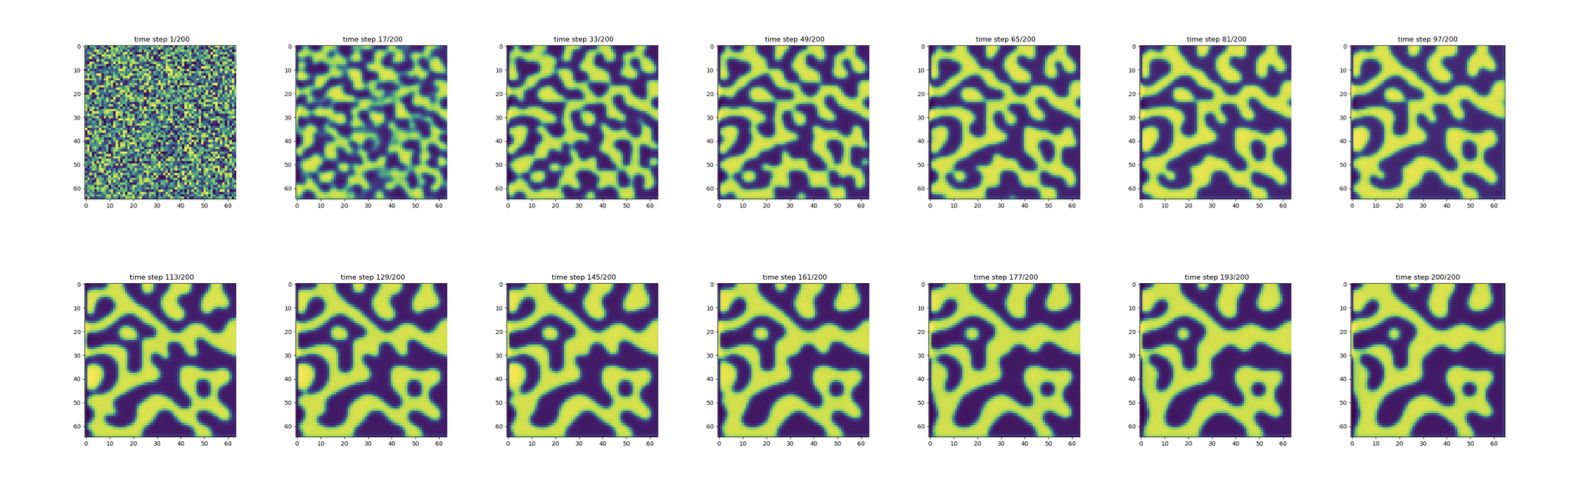
\includegraphics[scale=0.18]{phases/ch_phases.jpeg}
 \caption{phases transition}
 \label{fig:1}
\end{figure}
\end{frame}

\subsection{SAV with Fourier Transform for Allen-Cahn Equation}
\begin{frame}{Configuration and Main Idea}
\begin{itemize}
\item{Let $\mathcal G=-1, \mathcal L = -\Delta$, one gets the Allen-Cahn Equation from previous discussion}\item{The complexity of SAV mainly locates in solving equation of the form $$(I-\Delta t \mathcal{G L}) x = b$$}\item{I used Fourier Transfom to solve the above equation in the frequency domain and then inverse transform the result back to the phase field}
\end{itemize}
\end{frame}

\begin{frame}{Numerical Results}
\begin{itemize}
\item{I ran the above five schemes on $[0,1]^2 \times 20000\Delta t $, with smooth initial conditions $\phi_0(x,y) = 0.05 sin(2\pi x)sin(2\pi y)$, and the mesh resolution was set $128\times128$. The difference scheme was first order.}
\item{
 \begin{figure}[H]
  \centering
  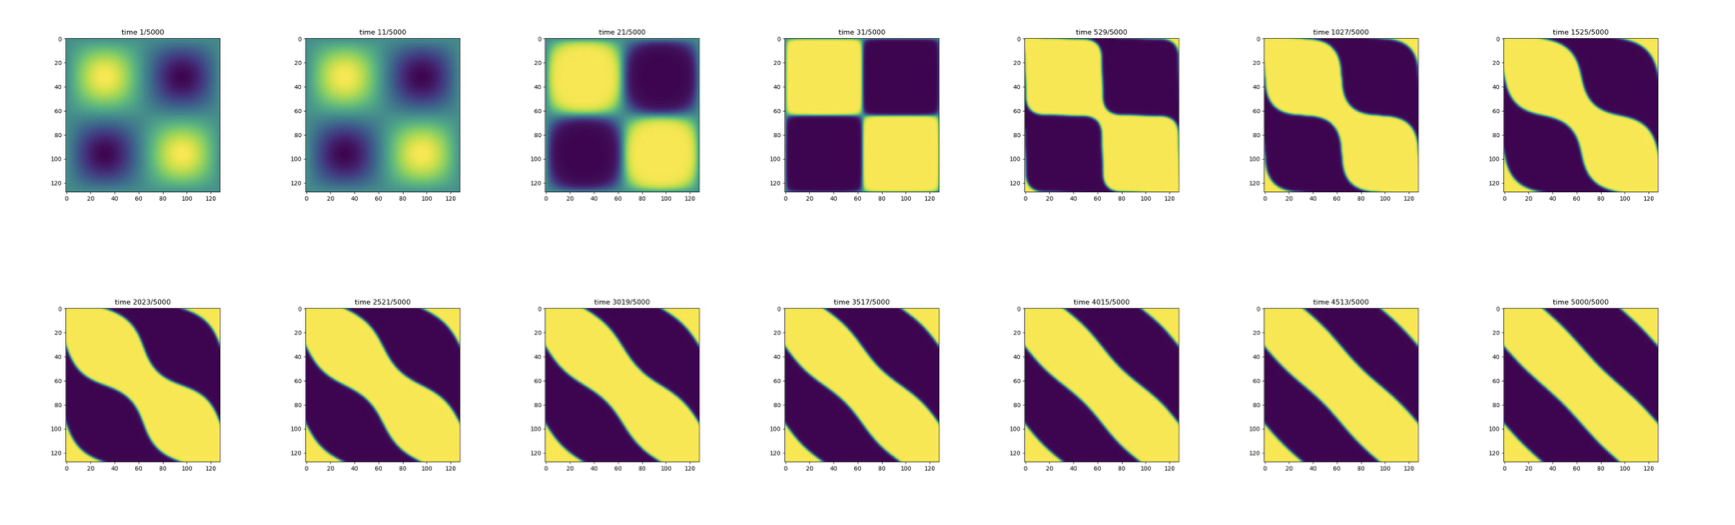
\includegraphics[scale=0.18]{phases/sav_phases.jpeg}
 \caption{phases transition}
 \label{fig:2}
\end{figure}
}
\end{itemize}
\end{frame}

\begin{frame}{Energy decay}
The modified and raw free energy changes as follow
 \begin{figure}[H]
  \centering
  \includegraphics[scale=0.35]{energy.jpg}
 \caption{Modified and Raw Free Energy}
 \label{fig:3}
\end{figure}
\end{frame}

\section{Code}

\begin{frame}
Related code is uploaded to

\url{https://github.com/burning489/cahn-hiliard} 

\url{https://github.com/burning489/sav}

Welcome further discussion :)

\end{frame}

\begin{frame}
 \begin{center}
{\huge \emph{\textcolor{cyan}{Thank you!}}}\\
\end{center}
\end{frame}

\nocite{*}
\begin{frame}[allowframebreaks]{References}
	\bibliographystyle{amsalpha}
	\bibliography{./beamer.bib}
\end{frame}

\end{document}
